\chapter{Anwendungen und Fallbeispiele}

\section{Fernerkundung und Vegetationsindizes}
Die spektralen Eigenschaften von Vegetation erlauben die Ableitung von Indizes, die Biomasse, Vitalität oder Stress erfassen. Ein klassisches Beispiel ist der \textit{Normalized Difference Vegetation Index} (NDVI):
\[
\mathrm{NDVI} = \frac{(\mathrm{NIR} - \mathrm{Rot})}{(\mathrm{NIR} + \mathrm{Rot})}
\]
Die physikalische Grundlage: starke Absorption im Roten durch Chlorophyll, hohe Reflexion im nahen Infrarot durch Blattgewebe und Streuung. Grenzen entstehen bei sehr hoher Blattfläche (Sättigung) und in heterogenen Mischpixeln. Die mechanistischen Zusammenhänge sind im Theoriekapitel erläutert \parencite{meyer2018photosynthese}.

\subsection{Beispiel: Wiesenmonitoring}
\begin{itemize}
  \item \textbf{Ziel}: Vitalitätsentwicklung einer Rasen- oder Wiesenfläche über die Saison.
  \item \textbf{Daten}: Multispektrale Aufnahmen (Rot, NIR) im Wochenabstand.
  \item \textbf{Auswertung}: NDVI-Zeitreihe; Identifikation von Trockenphasen (Abfall), Erholung (Anstieg).
\end{itemize}
\begin{figure}[H]
  \centering
  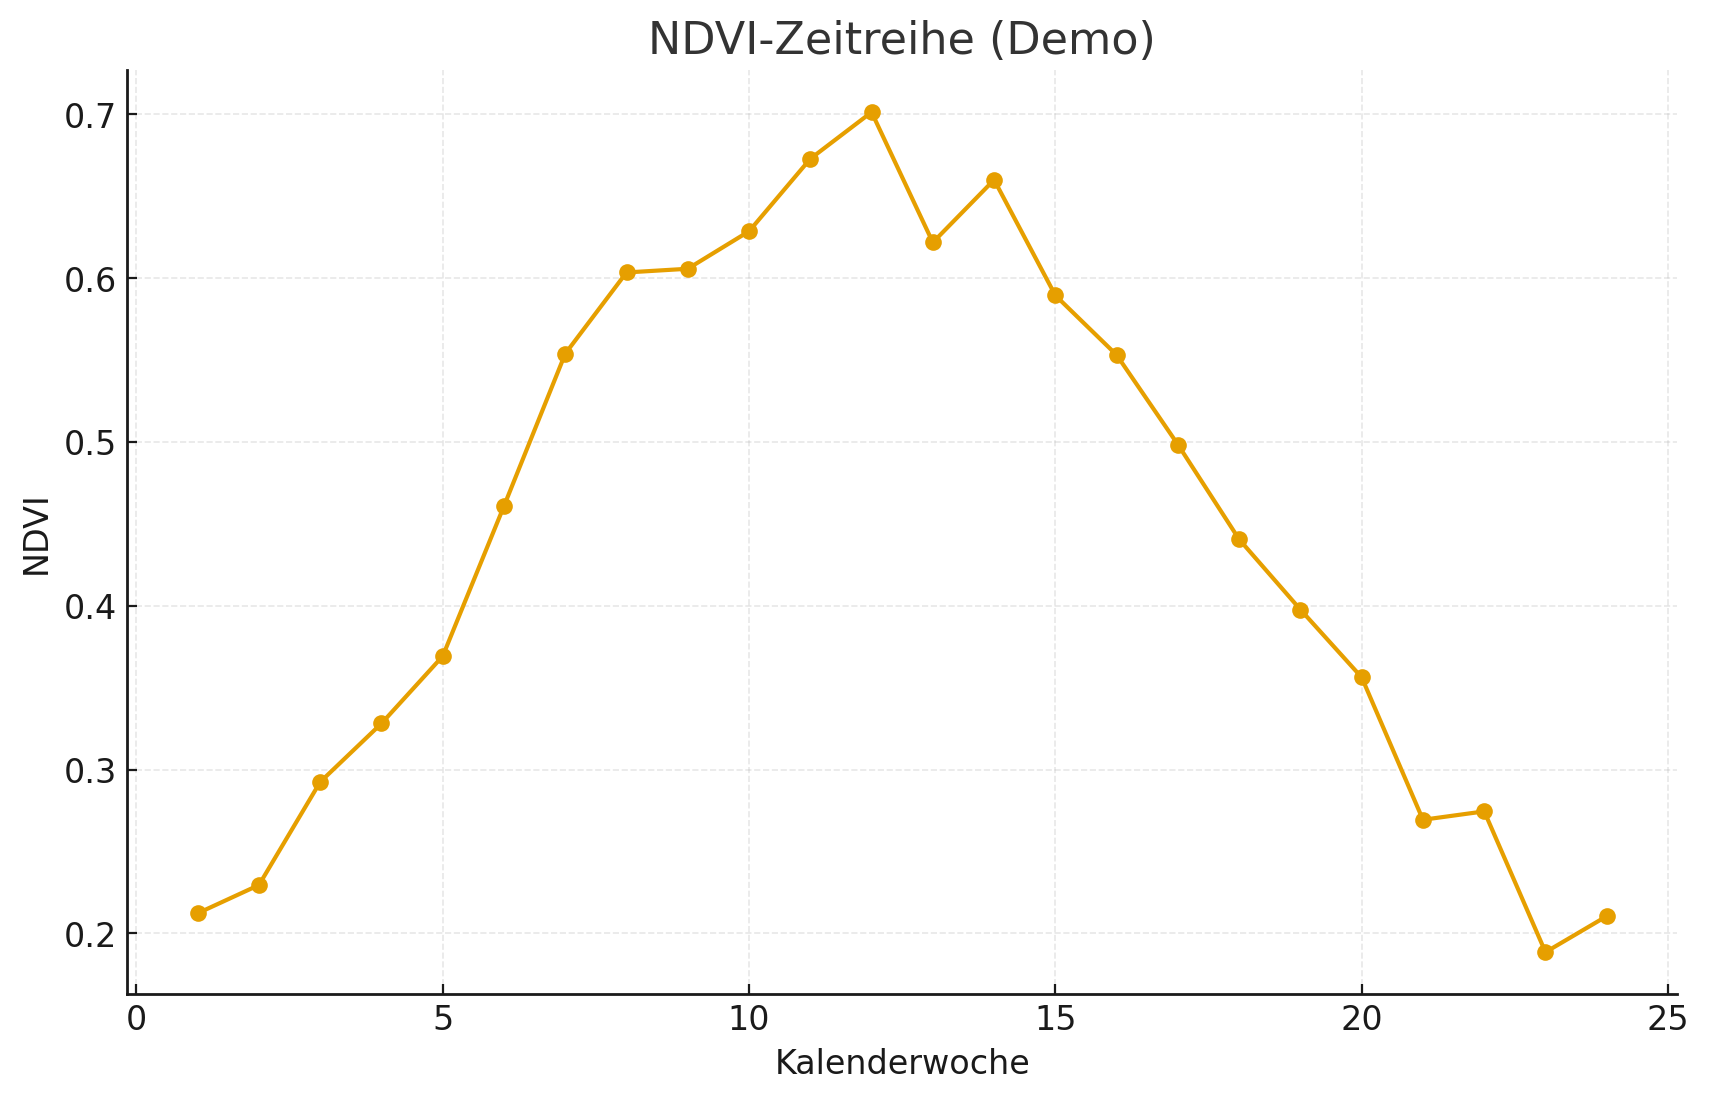
\includegraphics[width=.8\textwidth]{bilder/ndvi_demo.png}
  \caption{NDVI-Zeitreihe einer Beispielwiese. Platzhaltergrafik; bitte durch eigene Daten ersetzen.}
  \label{fig:ndvi}
\end{figure}

\section{Blatt- und Bestandsmessungen}
\subsection{Spektren am Blatt}
Reflexions- und Transmissionsmessungen zeigen die klassische „grüne Lücke“ sowie die starke Absorption im Blau und Rot. Änderungen der Pigmentgehalte verschieben die Kurven \parencite{meyer2018photosynthese}.
\begin{figure}[H]
  \centering
  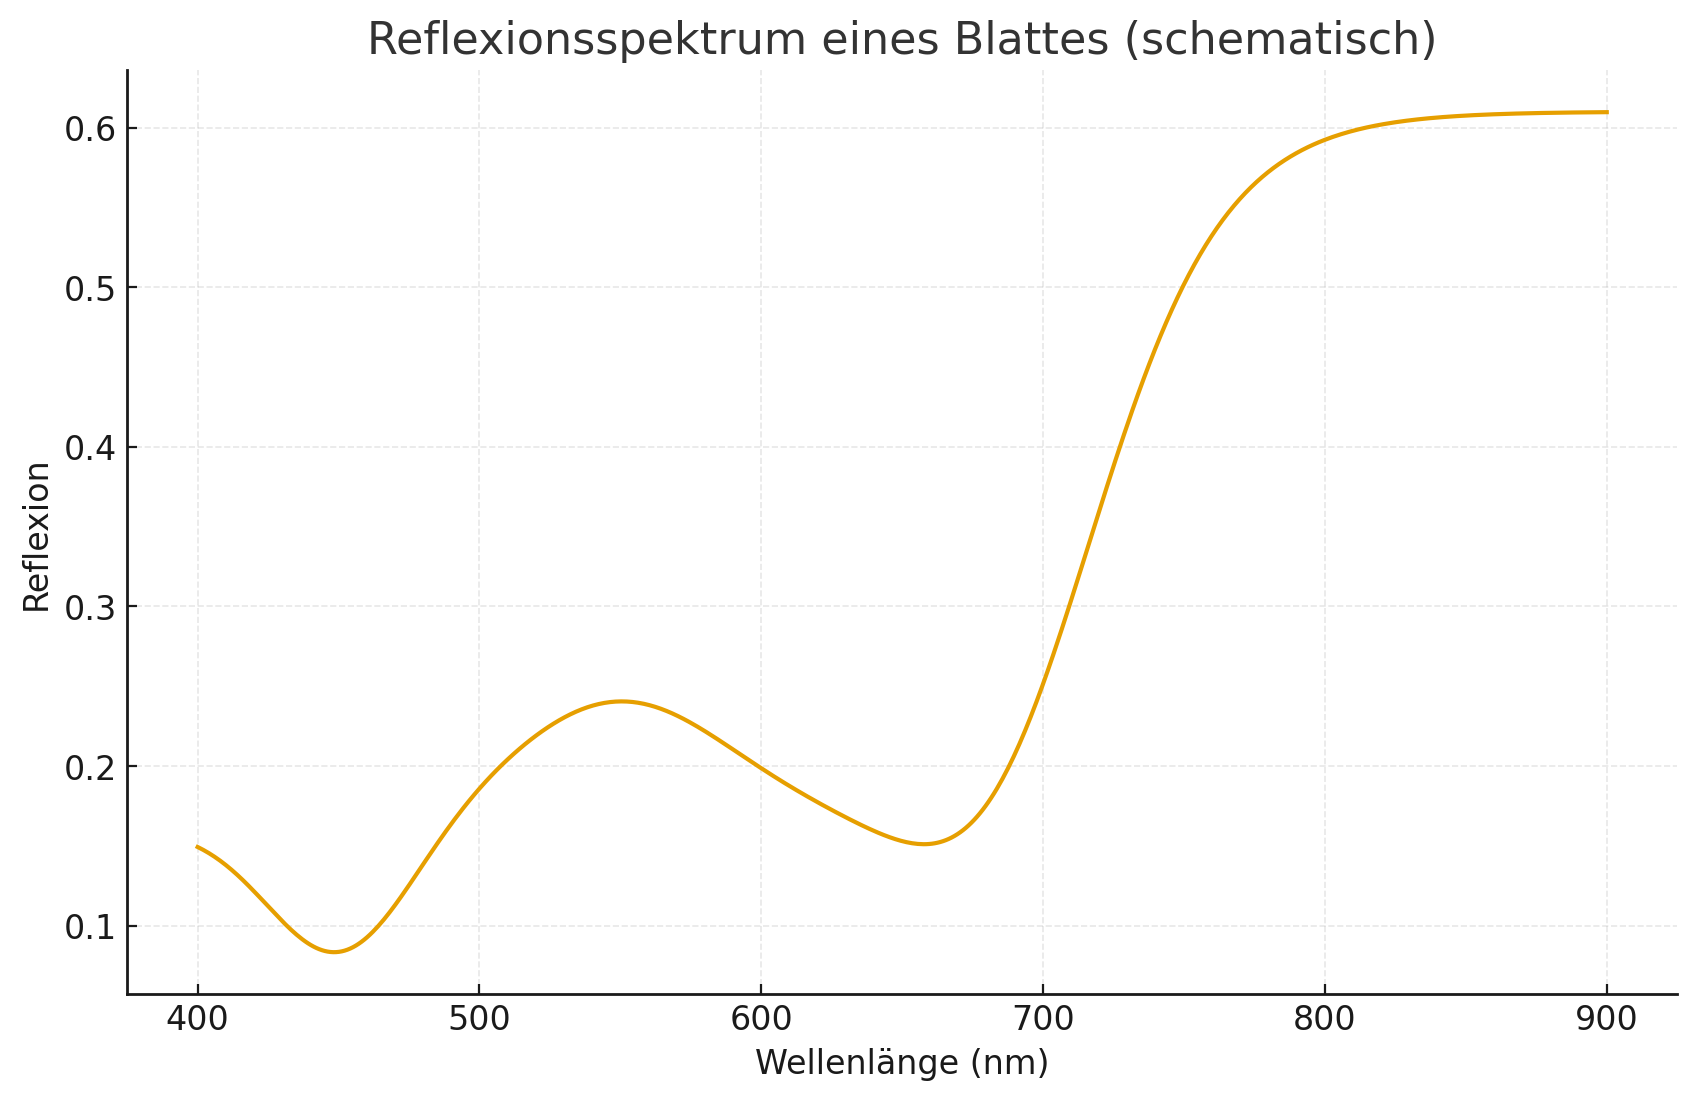
\includegraphics[width=.75\textwidth]{bilder/blattspektrum_demo.png}
  \caption{Reflexionsspektrum eines Blattes (schematisch). Platzhalter.}
  \label{fig:blatt_spektrum}
\end{figure}

\subsection{Chlorophyllfluoreszenz}
Die maximale Quantenausbeute der Photosysteme ($F_\mathrm{v}/F_\mathrm{m}$) dient als empfindlicher Stressindikator. Unter hoher Lichtlast oder Nährstoffmangel sinkt $F_\mathrm{v}/F_\mathrm{m}$ typischerweise; Photoprotektion stabilisiert das System \parencite{zhao2012chlorophyll, gao2010lightabsorption}.

\section{Fallbeispiele}
\subsection{Fall 1: Schatten vs. Sonne}
\textbf{Fragestellung}: Verändert sich die wahrgenommene Farbe und das Spektrum zwischen sonnigen und schattigen Bereichen?  
\textbf{Erwartung}: In Schattenlagen relativ höherer Grünanteil am einfallenden Licht; Blattanpassungen können zu veränderten Pigmentverhältnissen führen \parencite{zhao2012chlorophyll}.
\begin{figure}[H]
  \centering
  
\includegraphics[width=.8\textwidth]{bilder/schatten_sonne_foto.png}
  \caption{Beispielaufnahmen: Schatten- und Sonnenbereich einer Rasenfläche. Platzhalter.}
  \label{fig:schatten_sonne}
\end{figure}

\subsection{Fall 2: Trockenstress}
\textbf{Fragestellung}: Wie reagieren Farbe und Indizes auf Wasserdefizit?  
\textbf{Erwartung}: Abnahme blattgrüner Pigmente, steigende Braun-/Gelbtöne, fallender NDVI bzw. veränderte Reflexion \parencite{gao2010lightabsorption}.
\begin{figure}[H]
  \centering
  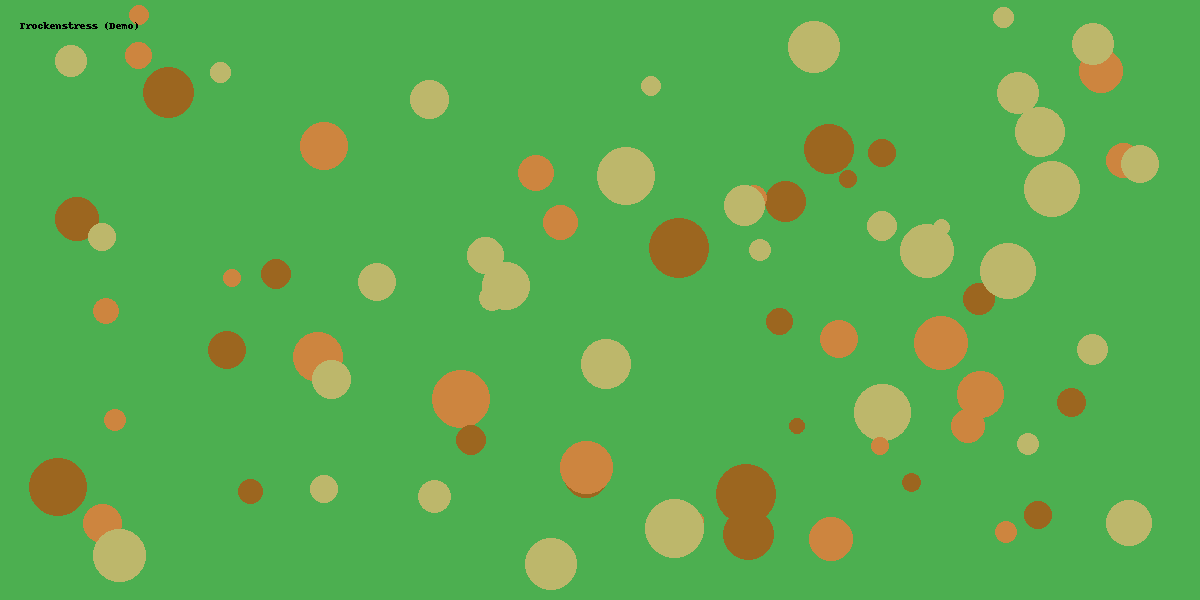
\includegraphics[width=.8\textwidth]{bilder/trockenstress_foto.png}
  \caption{Visuelle Veränderungen bei Trockenstress. Platzhalter.}
  \label{fig:trockenstress}
\end{figure}

\subsection{Fall 3: Düngung und Regeneration}
\textbf{Fragestellung}: Welche Veränderungen zeigen sich nach N-Düngung?  
\textbf{Erwartung}: Erhöhung des Chlorophyllgehalts, intensivere Grünfärbung, NDVI-Anstieg, ggf. höhere $F_\mathrm{v}/F_\mathrm{m}$ \parencite{schmidt2015chlorophyll}.
\begin{figure}[H]
  \centering
  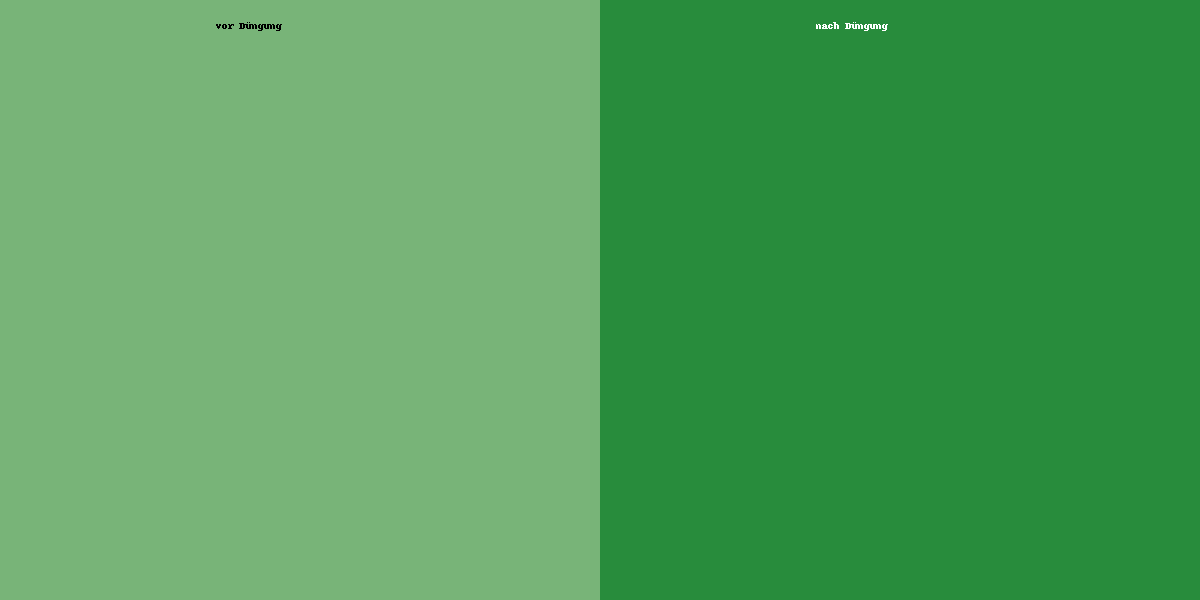
\includegraphics[width=.8\textwidth]{bilder/duengung_foto.png}
  \caption{Visuelle und spektrale Veränderungen nach Düngung. Platzhalter.}
  \label{fig:duengung}
\end{figure}

\section{Methodische Hinweise zur Reproduzierbarkeit}
\begin{itemize}
  \item \textbf{Dokumentation}: Datum, Uhrzeit, Wetter, Sonnenstand, Kameraparameter bzw. Sensorkalibration.
  \item \textbf{Referenzen}: Weißstandard/Referenztafel für Fotos; Spektronormierung für Messgeräte.
  \item \textbf{Auswertung}: Einheitliche Bildausschnitte; identische NDVI-Berechnung; Fehlerbalken für Zeitreihen.
\end{itemize}
